Arguably the biggest development in computing in the last few decades has been
the advent and proliferation of sensor driven
computing~\cite{krishnamurthi_overview_2020}.  Use of image, health, audio, and
other sensors have resulted in novel computing platforms such as
wearables~\cite{shamma2007watch}, head mounted
displays~\cite{jensen2018review}, and smartphones~\cite{smith2013smartphone},
and novel computing applications such as health and wellness
tracking~\cite{alslaity2022mobile}, digital navigation~\cite{vvcelak2005amr},
and extended reality~\cite{huzaifa2020exploring}. Indeed, each new class of
sensors can potentially enable new applications and generate new computational
requirements.

Different programmable computing platforms emerge at different times driven by
technology as well as applications. One programmable computing platform that
may be on the cusp of explosion is that of ``earables"~\cite{rethink} ---
devices such as earphones~\cite{boseearbuds, bosesports, sonyxm3}, hearing
aids~\cite{eargoneo}, and smart glasses~\cite{boseframe, amazonframe} that are
worn in or around the ear and that interact with humans mostly through
acoustics.  These devices have a large number of sensors~\cite{sensorsinear}
which can be leveraged to support a variety of applications
(Fig.~\ref{fig:earable_vision}).

\begin{wrapfigure}{L}{0.5\textwidth}
    \centering
    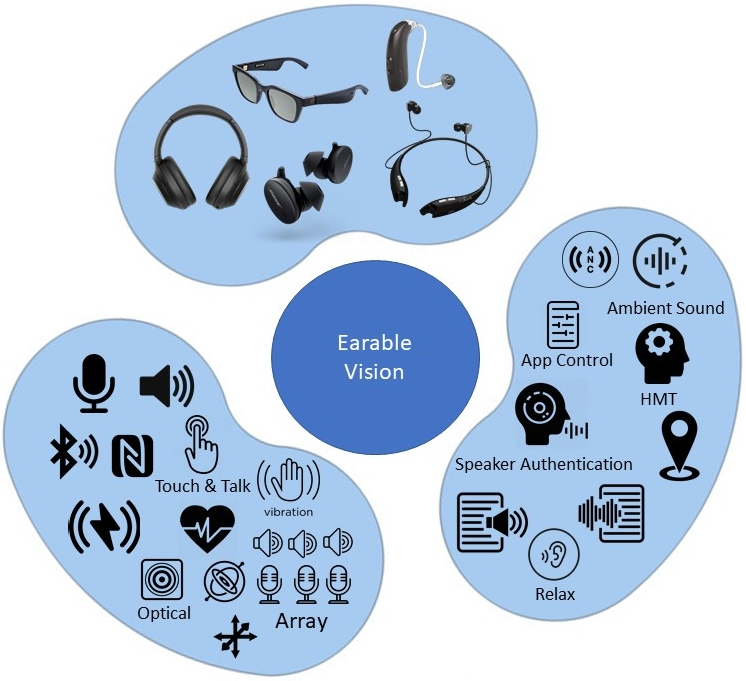
\includegraphics[width=\linewidth]{figs/vision_3.jpg}
    \caption{\small
        Emerging earable devices will be programmable platforms with a rich set
        of sensors and will support a variety of applications.
    }
    \label{fig:earable_vision}
\end{wrapfigure}

There are several signs that earables may become a prominent programmable
computing platform.  First, the current global market for earables is already
over 20 billion dollars and is expected to exceed 90 billion dollars in the
next three years~\cite{market}. Second, hardware vendors are already building
earables with increasingly complex sensors (e.g., proximity sensors,
gyroscopes, capacitive sensors, accelerometers, SpO2, EEG, EOG, EMG sensors,
microphone and speaker arrays, etc.) which are being leveraged to support a
wide variety of computing applications~\cite{jabra, earbleai, airpodsmax}.
Third, many earable platforms are already programmable and increasingly so.  In
fact, a large variety of software applications processing different sensor data
are already supported in many of today's earables~\cite{jabra, earableai,
airpodsmax} or are being explored~\cite{aptx, mute, petersn, earar}.  Fourth,
enabling technologies are increasingly production ready.  For example,
transformer networks have enabled super-human performance in natural language
understanding tasks, enabling smart audio interfaces between the earable device
and the user.

Earables as a computing platform may become popular also because acoustic
communication requires much less cognitive re-focus than visual or haptic
communication (e.g., using smartphones)\cite{rethink}. An earable is also a
better platform for sensing and analyzing upper body and head-based data,
compared to a phone or a watch, for example. Furthermore, unlike some other
wearables, most earables (e.g., earphones and hearing aids) already have social
acceptability and wide reach -- computing will simply be piggybacked on
these well-accepted devices.

Another class of sensor data processing that 
mae become 
%has been barely explored in the
mainstream is {\em \olfc{}}.  Smell has always received scant
recognition~\cite{rouby2002olfaction}, and has historically been considered an
inferior sense~\cite{rouby2002olfaction}, in spite of arguably being the most
visceral of senses~\cite{stewart_2022}. Biological understanding of odor has
also been relatively recent~\cite{nobelprize.org_2004}. Previous attempts at \olfc{}, in
the form of e-noses~\cite{karakaya2020electronic}, for example, have seen
limited success~\cite{smith_kiger_2006, platt_1999}, discouraging further
research and adoption; some attempts have indeed been publicly
ridiculed~\cite{smith_kiger_2006}. Finally, odor sensors that \olfc{} would
rely on have historically been highly inaccurate, power hungry, and
slow~\cite{wilson2016recent}; pumps and cartridges required for any odor
synthesis~\cite{olorama_technology, aromajoin_corporation, tillotson2006scent,
amores2017essence, anthrotronix_2019} application have been similarly big,
slow, and power hungry~\cite{mielle2022cold, solis2005fluctuation, maritex}.

\begin{wrapfigure}{r}{0.5\textwidth}
    \centering
    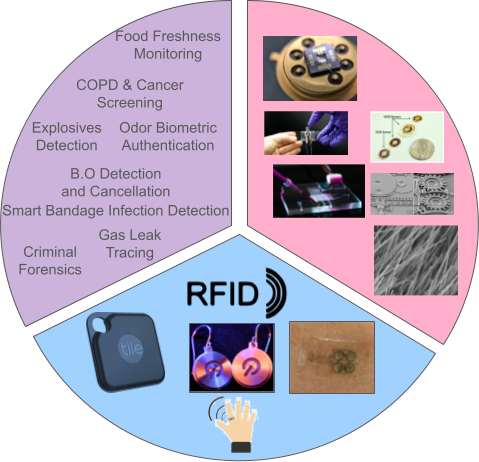
\includegraphics[width=0.7\linewidth]{./figs/odor_vision.png}
    \caption{\small
        An overview of \olfc{} applications,
        form-factors, and sensors \& actuators.
    }
    \label{fig:vision}
\end{wrapfigure}

In spite of the checkered history, we believe that this is a good time to
revisit \olfc{}. A large number of driver applications are emerging that would
require or benefit from \olfc{}. Low cost healthcare (e.g., smart bandages for
infection detection~\cite{derakhshandeh2018smart})  and personal hygiene
applications (body odor detection~\cite{wongchoosuk2009detection, jha2015quick,
jha2016gc, jha2015human}), for example, could benefit greatly when augmented
with odor sensing and synthesis. Second, there have been dramatic recent
advances in odor sensing technology, with some modern odor sensors
demonstrating high accuracy, miniatuarized to the micron scale, and consuming no
more than low tens of \si{\micro\watt} of power
(Fig.~\ref{fig:sensor_timelines}).  There have been similar advances in
NEMS/MEMS-based micropumps and cartridges~\cite{tillotson2006scent}.  Third,
widespread acceptance of sensor, wearable, and xR devices over the last decade,
including recent interest in odor-based wearable~\cite{olorama_technology,
tillotson2006scent, amores2017essence, anthrotronix_2019, peters_2019,
amores2018promoting, bahremand2022smell} and xR~\cite{stewart_2022} devices,
suggests a much easier path of adoption for \olfc{}-based applications than
ever before - overlaid on these devices. This vision of \olfc{} is
depicted in Fig.~\ref{fig:vision} which shows example odor applications, form
factors for \olfc{}-enabled devices, and odor sensors and actuators.


